%% Copyright 2007-2020 Elsevier Ltd
%% 
%% This file is part of the 'Elsarticle Bundle'.
%% ---------------------------------------------
%% 
%% It may be distributed under the conditions of the LaTeX Project Public
%% License, either version 1.2 of this license or (at your option) any
%% later version.  The latest version of this license is in
%%    http://www.latex-project.org/lppl.txt
%% and version 1.2 or later is part of all distributions of LaTeX
%% version 1999/12/01 or later.
%% 
%% The list of all files belonging to the 'Elsarticle Bundle' is
%% given in the file `manifest.txt'.
%% 
%% Template article for Elsevier's document class `elsarticle'
%% with harvard style bibliographic references

\documentclass[review,12pt,authoryear]{elsarticle}

%% Use the option review to obtain double line spacing
%% \documentclass[authoryear,preprint,review,12pt]{elsarticle}

%% Use the options 1p,twocolumn; 3p; 3p,twocolumn; 5p; or 5p,twocolumn
%% for a journal layout:
%% \documentclass[final,1p,times,authoryear]{elsarticle}
%% \documentclass[final,1p,times,twocolumn,authoryear]{elsarticle}
%% \documentclass[final,3p,times,authoryear]{elsarticle}
%% \documentclass[final,3p,times,twocolumn,authoryear]{elsarticle}
%% \documentclass[final,5p,times,authoryear]{elsarticle}
%% \documentclass[final,5p,times,twocolumn,authoryear]{elsarticle}

%% For including figures, graphicx.sty has been loaded in
%% elsarticle.cls. If you prefer to use the old commands
%% please give \usepackage{epsfig}

%% The amssymb package provides various useful mathematical symbols
\usepackage{amssymb}
%% The amsthm package provides extended theorem environments
%% \usepackage{amsthm}

%% The lineno packages adds line numbers. Start line numbering with
%% \begin{linenumbers}, end it with \end{linenumbers}. Or switch it on
%% for the whole article with \linenumbers.
\usepackage{lineno}

% for adjusting table width automatically
\usepackage{adjustbox}
\usepackage{tabulary, ragged2e}
\usepackage{booktabs}
\usepackage{multirow}

\usepackage{csvsimple}
\usepackage{longtable}
\journal{Geography and Sustainability}
%1.Full Length Article A full-length article should be a substantial and in-depth research study regarding a particular state of issue through several techniques or approaches. 
% The main text should be approximately 6,000 words in length, but it should not exceed 8,000 words (excluding abstract, references, tables, figures, and appendices).
%A maximum of 250 words abstract and up to 10 displayed items (figures and tables) is allowed. A full-length article should include an Introduction,
%Materials and methods, Results, Discussion, Conclusions, and References, which can be accompanied by Supplementary material.

\begin{document}
\begin{linenumbers}
\begin{frontmatter}
%% Title, authors and addresses
%% use the tnoteref command within \title for footnotes;
%% use the tnotetext command for theassociated footnote;
%% use the fnref command within \author or \affiliation for footnotes;
%% use the fntext command for theassociated footnote;
%% use the corref command within \author for corresponding author footnotes;
%% use the cortext command for theassociated footnote;
%% use the ead command for the email address,
%% and the form \ead[url] for the home page:
%% \title{Title\tnoteref{label1}}
%% \tnotetext[label1]{}
%% \author{Name\corref{cor1}\fnref{label2}}
%% \ead{email address}
%% \ead[url]{home page}
%% \fntext[label2]{}
%% \cortext[cor1]{}
%% \affiliation{organization={},
%%            addressline={}, 
%%            city={},
%%            postcode={}, 
%%            state={},
%%            country={}}
%% \fntext[label3]{}
\title{The influence of resource use on yield versus sale price trade-off in Australian vineyards}
%% use optional labels to link authors explicitly to addresses:
%% \author[label1,label2]{}
%% \affiliation[label1]{organization={},
%%             addressline={},
%%             city={},
%%             postcode={},
%%             state={},
%%             country={}}
%%
%% \affiliation[label2]{organization={},
%%             addressline={},
%%             city={},
%%             postcode={},
%%             state={},
%%             country={}}
%\affiliation[label1]{organization={QUT},
%  addressline={},
%  city={},
%  postcode={},
%  state={QLD},
%  country={}}
%\affiliation[label2]{organization={AWRI},
%  addressline={},
%  city={},
%  postcode={},
%  state={SA},
%  country={}}
%\affiliation[label3]{organization={Food Agility CRC},
%  addressline={},
%  city={},
%  postcode={},
%  state={Vic},
%  country={}}
\author[label1,label2,label3]{Author}
\date{02/08/2023}
\begin{abstract}
% The word limit needs to be checked.
When strategies for a sustainable winegrowing industry are assessed, there is a trade-off between balancing the amount of resources invested and the resultant yield and sale price of the produce. In this analysis we observe relationships between resource use, yield and sale price through the use of statistical models. The dataset used for this analysis includes data collected for the past 10 years from 1261 vineyards located over a diverse range of Australian winegrowing regions. Yield and sale price was modelled to resource factors related to water use and Green House Gas (GHG) emissions. The analysis confirmed a strong relationship between area and resource use, with the overall area of a vineyard and its access to resources greatly determining the upper limit of yield. However, area was also negatively related to the average sale price of grapes, we find that higher average sale prices were connected to high resource inputs per area; rather than to the overall expenditure of resources. Regional and temporal effects on vineyard yield and average sales price were also identified. Overall, the analysis highlighted the importance of considering a vineyard's business goal, region, external pressures and economies of scale, when considering whether to pursue higher yields or average sales prices.
\end{abstract}
%%Graphical abstract`
%\begin{graphicalabstract}
 % 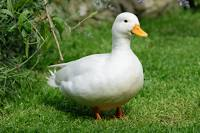
\includegraphics{graphical_abstract.jpeg}
%\end{graphicalabstract}'

%\begin{keyword}
%% keywords here, in the form: keyword \sep keyword
%Keyword one \sep{} keyword two
%% PACS codes here, in the form: \PACS code \sep code
%\PACS{} 0000 \sep{} 1111
%% MSC codes here, in the form: \MSC code \sep code
%% or \MSC[2008] code \sep code (2000 is the default)
%\MSC{} 0000 \sep{} 1111
%\end{keyword}
%%Research highlights
\begin{highlights}
  \item Comparative analysis of resource use, average sale price and quantity in Australian winegrowing.
  \item Regional comparison of outcomes and resource use in Australian winegrowing regions.
  \item Baseline models for comparing vineyards.
  \item Analysis of national, decade long data source.
\end{highlights}
\end{frontmatter}

%%%%%%%%%%%%%%%%%%%%%%%%%%%%%%%%%%%%%%%%%%
%%                main text             %%
%%%%%%%%%%%%%%%%%%%%%%%%%%%%%%%%%%%%%%%%%%

\section{Introduction}
The global focus on sustainability in agronomic industries has changed the way in which these enterprises do business. A dilemma exists across agriculture through shared fundamental considerations of resource use such as water and fuel, and the resultant yield and crop value that is produced\citep{hemmingCherryTomatoProduction2020,kawasakiQualityMattersMore2016, zhuEffectsNitrogenLevel2017}. The average price of grapes for wine production is driven through its integration within the wine industry. An important connection between grapes and their price is the grapes perceived quality, which initially defines a wines potential through the grapes chemical makeup \citep{blackTerpenoidsTheirRole2015,schreierFlavorCompositionWines1979}. Grapes of higher of perceived quality or grapes from particularly famous regions are likely to have higher prices \citep{wineaustraliaNationalVintageReport2021}.  Grape quality is connected to the market value of winegrapes, with Wine Australia explicitly defining grape quality through the use of discrete price brackets in their annual reports \citep{winemakersfederationofaustraliaNationalVintageReport2018}. Although it is also important to note that the generalisation made to reflect quality through using average price assumes a due diligence of those who purchasing the grapes \citep{yeggeInfluenceSensoryNonsensory2001}. The economic sustainability of a vineyard is tied to this market culture driven by the wine industry. The consideration of sustainability within viticulture is also subject to environmental and socio-demographic pressures \citep{santiago-brownSustainabilityAssessmentWineGrape2015}. In the Australian context, these pressures include biosecurity and climate and international market changes \citep{canadellMultidecadalIncreaseForest2021,longbottomRoleVineyardPractices2015,oliverReviewSoilPhysical2013}.
\par
There is an extensive amount of research into the varied effects of factors on grape quality and yield \citep{heFruitYieldPrediction2022,laurentLocalInfluenceClimate2022,liakosMachineLearningAgriculture2018}. With there being a lack of research on grape sale price and its driving factors due to the lack of long-term and in-depth data. Furthermore, individual factors are often studied in isolation with yield and sales price not appearing together \citep{abbalDecisionSupportSystem2016}. The lack of consolidated datasets restricts the ability to gain statistical insights at large scales and across multiple regions, as a result broader studies are lacking \citep{keithjonesAustralianWineIndustry2002,knightFirmResourcesDevelopment2019}. The dataset used for this analysis includes data spanning 10 years from a multitude of vineyards located over a diverse range of Australian winegrowing regions. We use this dataset to describe the relationship of resources related to water and fuel use with the output yield and average sale price of the resultant product, taking into account the size and location of the vineyard. The practical addition of this aim is a baseline for comparison: given a vineyard within Australia, one could estimate the comparative efficiency with regard to the tradeoff between invested resources, yield and average sale price. This is the first time that such a trade off has been confirmed explicitly across such varying regions, scales and climates in the Australian winegrowing industry.
\section{Methods}
\subsection{Data}

\begin{table}[]
\caption{Summary of models; their predictors, covariates and variable interactions.}\label{tab:tab1}
  \resizebox{\textwidth}{!}{\begin{tabular}{@{}ccccc@{}}
    \toprule
    & \textbf{Response} & \textbf{Predictors} & \textbf{Covariates} & \textbf{Interactions} \\ \midrule
    \textbf{Model 1} & Yield & \begin{tabular}[c]{@{}c@{}}Water Used\\ scope one Emissions\end{tabular} & \begin{tabular}[c]{@{}c@{}}Area Harvested\\ Year\\ GI Region\end{tabular} & N/A \\
    \multicolumn{1}{l}{} & \multicolumn{1}{l}{} & \multicolumn{1}{l}{} & \multicolumn{1}{l}{} & \multicolumn{1}{l}{} \\
    \textbf{Model 2} & ${ \textrm{Yield}}\over{ \textrm{Area Harvested}}$ & \begin{tabular}[c]{@{}c@{}}Water Used\\ scope one Emissions\end{tabular} & \begin{tabular}[c]{@{}c@{}}Area Harvested\\ Year\\ GI Region\end{tabular} & \begin{tabular}[c]{@{}c@{}}Area Harvested * scope one Emissions\\ Area Harvested * Water Use\\ Year * Region\end{tabular} \\
    \multicolumn{1}{l}{} & \multicolumn{1}{l}{} & \multicolumn{1}{l}{} & \multicolumn{1}{l}{} & \multicolumn{1}{l}{} \\
    \textbf{Model 3} & {$\textrm{Yield} {\times} \textrm{Average Sale Price}$} & \begin{tabular}[c]{@{}c@{}}Water Used\\ Scope One Emissions\end{tabular} & \begin{tabular}[c]{@{}c@{}}Area Harvested\\ Year\\ GI Region\end{tabular} & N/A\\
    \multicolumn{1}{l}{} & \multicolumn{1}{l}{} & \multicolumn{1}{l}{} & \multicolumn{1}{l}{} & \multicolumn{1}{l}{} \\
    \textbf{Model 4} & Average Sale Price & \begin{tabular}[c]{@{}c@{}}Water Used\\ Scope One Emissions\end{tabular} & \begin{tabular}[c]{@{}c@{}}Area Harvested\\ Year\\ GI Region\end{tabular} & \begin{tabular}[c]{@{}c@{}}Area Harvested * Scope One Emissions\\ Area Harvested * Water Use\\ Year * Region\end{tabular}
        \\
        \multicolumn{1}{l}{} & \multicolumn{1}{l}{} & \multicolumn{1}{l}{} & \multicolumn{1}{l}{} & \multicolumn{1}{l}{} \\
     \textbf{Model 5} &  Average Sale Price & \begin{tabular}[c]{@{}c@{}}Water Used\\ Scope One Emissions\end{tabular} & \begin{tabular}[c]{@{}c@{}} Year\\ GI Region\end{tabular} & \begin{tabular}[c]{@{}c@{}} Year * Region\end{tabular}
        \end{tabular}}
\end{table}

Data used in these analyses were obtained from Sustainable Winegrowing Australia and Wine Australia. Sustainable Winegrowing Australia is Australia's national wine industry sustainability program, which aims to facilitate grape-growers and winemakers in demonstrating and improving their sustainability \citep{swaSustainableWingrowingAustralia2022}. Data collected by Sustainable Winegrowing Australia is entered voluntarily by winegrowers at the end of harvest. Wine Australia is an Australian Government statutory authority governed by the Wine Australia Act \citep{attorney-generalsdepartmentWineAustraliaCorporation2010}. Data collected by Wine Australia is publicly available.
\par
Predicted variables in this analysis were yield, defined as the total tonnes of grapes harvested, and average sale price of grapes. Both response variables were examined as totals and as scales of area harvested. Values were compared in this manner to observe how economies of scale affect the use of resources.
\par
Data obtained from Wine Australia were collected via phone surveys and included: total tonnes purchased, average price per tonne and yearly change in price for region and grape varietal. Data recorded by Sustainable Winegrowing Australia was entered manually by winegrowers using a web based interface with some fields being optional. Required variables included: region, harvest year, yield and area harvested. Harvest year and region were recorded as categorical variables. Optional variables included average sale price, water used and fuel used (diesel, petrol, biodiesel and LPG). The dataset was limited to respondents that recorded values for area harvested, water used, yield and fuel use. To enable direct comparisons between fuels, fuel use was converted to tonnes of Carbon Dioxide equivalent and collectively referenced to as emissions.
\par
Average sale price was an optional field in the Sustainable Winegrowing Australia's dataset. Missing values were improved using regional average prices from Wine Australia. Two subsets of data were then created for the analysis. The first subset contained all vineyards and was used for two models (Model 1 and Model 2, see Table \ref{tab:tab1}). The second subset contained vineyards which either recorded a value for average price of sale per tonne through Sustainable Winegrowing Australia, or were within a region with an average price of sale recorded by Wine Australia; this subset was used for three further models (Models 3, 4 and 5, see Table \ref{tab:tab1}). These subsets meant that the data would be limited to samples which had recorded values for the response variables (see Table \ref{tab:tab1}), where every sample had a recorded value for yield but not average price of sale per tonne.
\par
The first subset of data (used for Model 1 and Model 2, see Table \ref{tab:tab1}) contained 5298 samples spanning the period from 2012 to 2022, covering 55 GI Regions and 1261 discrete vineyards.
\par
The second subset of data (used for Model 3, Model 4 and Model 5, see Table \ref{tab:tab1}) contained 2878 samples spanning the period from 2015 to 2022, covering 51 GI Regions and 944 separate vineyards.Average price of sale per tonne was extracted from both Wine Australia (1842 values) and Sustainable Winegrowing Australia (remaining 1036 values).
\par
Additional variables were considered for analysis but were excluded due to being either underreported or had insignificant contributions to model accuracies. Variables explored but not used due to low reporting values included fertiliser, electricity, and scope two emissions. Variables considered but ultimately removed due to a lack of significant contributions to models, included the use of renewable energy, contractor use, and pressures such as frost, fire and disease.
\par
Data preprocessing was conducted prior to analysis using the Python programming language \citep{g.vanrossumPythonTutorialTechnical1995}. Preprocessing included the conversion from fuel to scope one emissions and prior calculations for all continuous variables which included logarithmic transformations, centring and scaling by standard deviation. 
We converted multiple emission sources into scope one emissions using the equation given from the Australian National Greenhouse Accounts Factors \citep{agdeeNationalGreenhouseAccounts2021}, shown as
\par
\begin{equation}
\label{(1)}
    tCO_{2}e={{Q \times EC \times EF1 + EF3}\over{1000}},
\end{equation}
\par
was used to convert the quantity of fuel in litres, $Q$, using a prescribed Energy Content, $EC$, and emission factors of scope one, $EF1$, and scope three, $EF3$, to tonnes of Carbon Dioxide Emission equivalent, $tCO2e$ \citep{departmentofclimatechangeenergytheenvironmentandwaterAustralianNationalGreenhouse2022}.
\par

\begin{figure}
  \resizebox{\textwidth}{!}{
  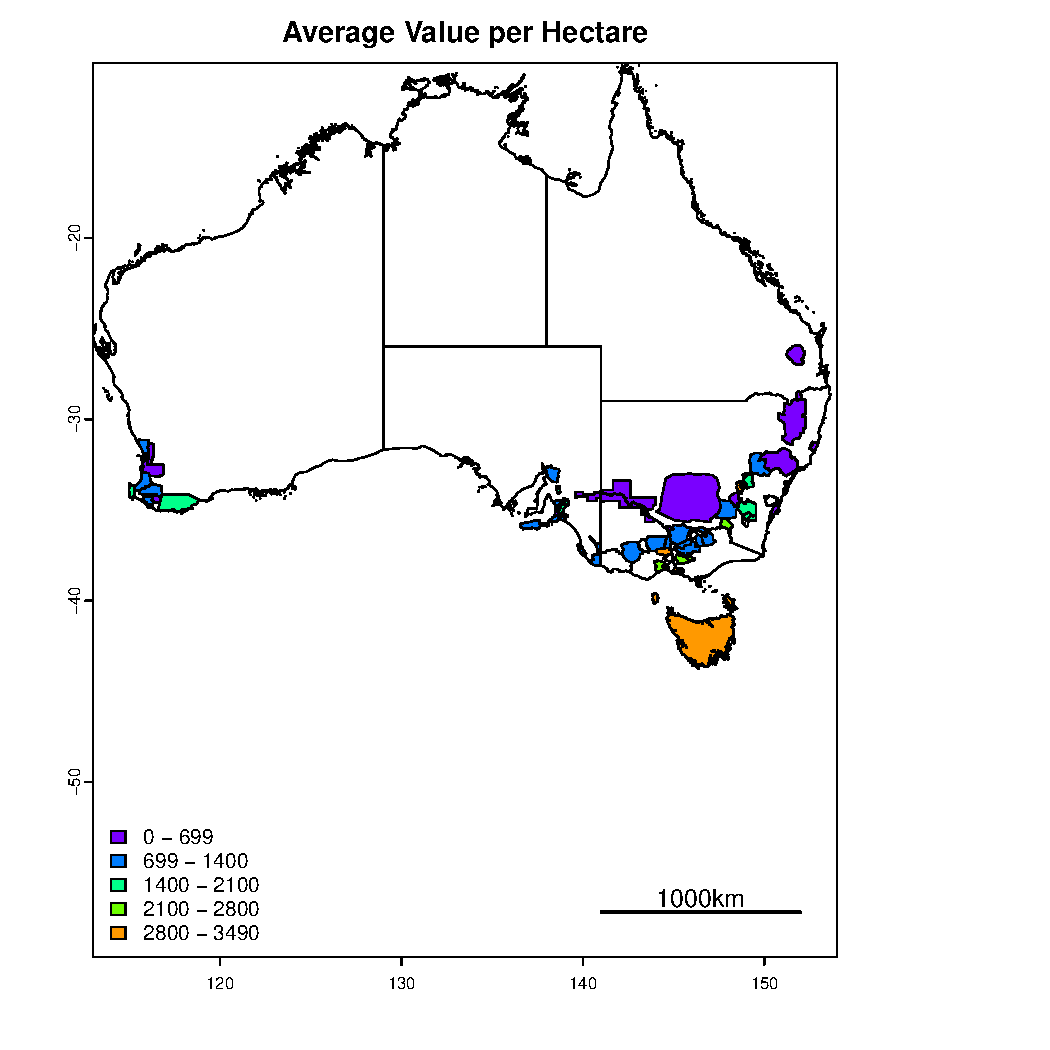
\includegraphics{my_map.pdf}}
  \caption{Map of each GI Regions average income for a vineyard of that region (average grape sale price per tonne $\times$ total tonnes yielded).}\label{fig:map}
\end{figure}%%

\par
The site of a vineyard predetermines several physical parameters such as climate, geology and soil, making location a widely considered key determinant of grape yield and average sale price \citep{abbalDecisionSupportSystem2016,agostaRegionalClimateVariability2012,fragaMultivariateClusteringViticultural2017}. Differences in vineyard locations were captured through the use of Geographical Indicator Regions (GI Regions, see Figure \ref{fig:map}) defined by Wine Australia \citep{hallidayAustralianWineEncyclopedia2009,oliverReviewSoilPhysical2013,soarClimateDriversRed2008}. Each GI Region has its own unique mixture of climatic and geophysical properties that describes a unique winegrowing region within Australia and is a protected trademark under the Wine Australia act \citep{attorney-generalsdepartmentWineAustraliaCorporation2010}. Both Wine Australia and Sustainable Winegrowing Australia used the same GI Region categorical variable format to describe location.
\par
 The climatic properties of each GI Region were summarised by using predefined classifications as per the \citet{sustainablewinegrowingaustraliaSustainableWinegrowingAustralia2021} user manual. The user manual describes climates by rainfall and temperature, creating supersets of Regions of similar climatic properties. The climatic groups were used to illustrate similarities and differences occurring in areas larger than GI Regions.
\par
\subsection{Analysis}
Pairwise Pearson Correlation Coefficients were calculated to assess the potential existence of linear relationships between the input and predicted variables. To determine if a coefficient was indicative of a strong relationship, confidence intervals were used. P-values reflected the significance of a given correlation coefficient with statistical significance being declared when the associated value was lower than 0.05. Pairwise Pearson Correlation Coefficients were calculated for data on the original scale and for data as a logarithmic transform. Transforming data prior to calculating the coefficients changes several things. The logarithmic transform of the data alters the interpretation of the coefficients to percentage change; a coefficient will be indicative of the change in percentage of one variable compared to the other, scaling by standard deviation also changes this interpretation to be a percentage of that variables standard deviation. When considering the logarithmically transformed variables, a coefficient of 1 would indicate that the change of one variable by one percentage of its standard deviation would correlate to the other variable changing by one percent of its own standard deviation. The importance of this is the dimensionless nature of these relationships and that it can be translated directly to any vineyard's case that has a well known distribution.
\par
Five general linear models were created (see Table \ref{tab:tab1}). Both the Pearson Correlation Coefficients and General Linear Models were created using the R statistical programming language \citep{rcoreteamLanguageEnvironmentStatistical2021} with the Caret package \citep{kuhnBuildingPredictiveModels2008}. General Linear Models were chosen as they offer the ability to produce statistical models that are explicit in the relationships between predictors and response variables.  General Linear Models also allowed the exploration of interactions between predictors and allow for easily comparable differences in the influence and magnitude of relationships. Model fit was measured in $R^2$ and adjusted $R^2$ as well as F statistics. T-tests were used to determine if predictors significantly contributed to their models when accounting for other variables, showing which specific years and areas contributed significantly. 
\par
A variety of alternate methods were also explored, including splines, hierarchical regression, General Additive Models, and Generalised Linear Models. These alternative approaches were not used as final models due to offering no further insights or improvements in accuracy.
\par
\subsection{Model Validation}
Models were validated using K-fold cross validation calculated. K-fold cross validation works by removing a subset of data from the sample used to train models and then predicts those variables to determine how sensitive the model is to changes in the sample data . For this analysis each model was validated using 10 folds, repeated 100 times.
\par
\section{Results}
\subsection{Exploratory Analysis}\label{sec:exp_anal}
 Table \ref{tab:summary} shows the summary statistics of each variable in its original units. The range of these values shows the level of difference between some vineyards, with operations differing by orders of magnitude in size, yield and average price of sale (See Table \ref{tab:tab1}).
\par
\begin{table}[]
  \caption{Summary statistics of each continuous variable.}\label{tab:summary}
      % \resizebox{\textwidth}{!}{
        \begin{tabular}{@{}cllll@{}}
          \toprule
          \textbf{Variable} & \textbf{Mean} & \textbf{\begin{tabular}[c]{@{}l@{}}Standard\\ Deviation\end{tabular}} & \textbf{Minimum} & \textbf{Maximum} \\ \midrule
          {Yield (tonnes)} & 7.757E+02 & 2.179E+03 & 1.000E+00 & 7.231E+04 \\
          \multicolumn{1}{l}{} &  &  &  &  \\
          {Area Harvested (ha)} & 6.670E+01 & 1.337E+02 & 7.000E-02 & 2.436E+03 \\
          \multicolumn{1}{l}{} &  &  &  &  \\
          {Water Used (ML)} & 7.471E+06 & 5.646E+08 & 1.000E+00 & 4.268E+10 \\
          \multicolumn{1}{l}{} &  &  &  &  \\
          {Scope One Emissions ($tCO_{2}e$)} & 4.173E+04 & 8.571E+04 & 6.755E+00 & 2.110E+06 \\
          \multicolumn{1}{l}{} &  &  &  &  \\
          $\mbox{Yield (tonnes)}\over \mbox{Area harvested (ha)}$ & 1.009E+01 & 8.127E+00 & 4.000E-02 & 8.634E+01 \\
          \multicolumn{1}{l}{} &  &  &  &  \\
          {Average Sale Price (AUD/tonne)} & 1.477E+03 & 9.216E+02 & 1.600E+02 & 2.600E+04 \\
          \multicolumn{1}{l}{} &  &  &  &  \\
          $\mbox{Average Sale Price (AUD/tonne)} \over \mbox{Area Harvested (ha)}$ & 1.347E+02 & 5.711E+02 & 1.753E-01 & 2.979E+04 \\ \bottomrule
          \end{tabular}
  % }
  \end{table}

Pearson Correlation Coefficients of the transformed, centred and scaled variables are shown in Table \ref{tab:pearson_correlation}. All correlations were found to be statistically significant (P $<$ 2.200E-16), and except for 'average price' all variables were positively correlated. With water use, area harvested and emissions being positively correlated to yield, it can be considered that more resources and area are likely to lead to greater yields. Average sale price's negative correlation to yield, water use, area and scope one emissions, indicated that size and fuel separately were not the determining factor for average sale price. The negative correlations are not causal relationships but relative (using more water does not cause lower sale prices).
\par
\begin{table}[]
  \caption{Pairwise Pearson correlation coefficients for logarithmically transformed values.}\label{tab:pearson_correlation}
      \resizebox{\textwidth}{!}{
      \begin{tabular}{@{}cccccccc@{}}
          \toprule
          \textbf{} & \multicolumn{1}{c}{\textbf{Yield}} & \multicolumn{1}{c}{\textbf{Area Harvested}} & \multicolumn{1}{c}{\textbf{Water Used}} & \multicolumn{1}{c}{\textbf{\begin{tabular}[c]{@{}c@{}}Scope One\\ Emissions\end{tabular}}} & \multicolumn{1}{c}{\textbf{\begin{tabular}[c]{@{}c@{}}Yield by\\ Area\end{tabular}}} & \multicolumn{1}{c}{\textbf{Average Price}} & \multicolumn{1}{c}{\textbf{\begin{tabular}[c]{@{}c@{}}Average Price\\ by Area\end{tabular}}} \\ \midrule
          Yield & 1.00 & 0.88 & 0.82 & 0.76 & 0.96 & -0.46 & -0.88 \\
          Area Harvested & 0.88 & 1.00 & 0.78 & 0.83 & 0.73 & -0.19 & -0.81 \\
          Water Used & 0.82 & 0.78 & 1.00 & 0.67 & 0.76 & -0.49 & -0.82 \\
          \begin{tabular}[c]{@{}c@{}}Scope One\\ Emissions\end{tabular} & 0.76 & 0.83 & 0.67 & 1.00 & 0.65 & -0.16 & -0.67 \\
          \begin{tabular}[c]{@{}c@{}}Yield by\\ Area\end{tabular} & 0.96 & 0.73 & 0.76 & 0.65 & 1.00 & -0.54 & -0.84 \\
          Average Price & -0.46 & -0.19 & -0.49 & -0.16 & -0.54 & 1.00 & 0.72 \\
          \begin{tabular}[c]{@{}c@{}}Average Price\\ by Area\end{tabular} & -0.88 & -0.81 & -0.82 & -0.67 & -0.84 & 0.72 & 1.00 \\ \bottomrule
          \end{tabular}}
\end{table}

\subsection{General Linear Models}

Each model had a high $R^2$ value, indicating that most of the variance within the data was described by the models (see Table~\ref{tab:modelsummary}). The models were found to be a good fit, with overall F-tests being statistically significant (P $<$ 2.200E-16). And, aside from 3 variables, F-tests across each model's variables were also significant (with all being at least, P $<$ 0.05). The three exceptions were: scope one emissions in Model 3 (P=0.22) and Model 4 (P=0.0.39), and the interaction between area harvested and water used in model 2 (P=0.22). Note that, scope one emissions was included in all models to directly compare the response variables as ratios of vineyard size to raw values and because it was strongly correlated to the response variable in every model (except model 5); especially for Models 1 and 4 (Table \ref{tab:pearson_correlation}). 
%A full list of regression coefficients 95\% CIs and p-values for each of the four models is provided in the appendix. % You gotta add these to the appendix in a more readable fashion
\par
\begin{table}[]
  \caption{Summary of models; their performance, F-statistics and Residual error.}\label{tab:modelsummary}
      \resizebox{\textwidth}{!}{
        \begin{tabular}{@{}cccccccc@{}}
          \toprule
           & $\mathbf{R^2}$ & \textbf{\begin{tabular}[c]{@{}c@{}} Adjusted\\ $\mathbf{R^2}$ \end{tabular}} & \textbf{F-Statistic} & \textbf{P-Value} & \textbf{\begin{tabular}[c]{@{}c@{}}Residual\\ Standard Error\end{tabular}} & \textbf{\begin{tabular}[c]{@{}c@{}}Residual Sum\\ of Squares\end{tabular}} & \textbf{\begin{tabular}[c]{@{}c@{}}Residual Mean\\ of Squares\end{tabular}} \\ \midrule
          \textbf{\begin{tabular}[c]{@{}c@{}}Model 1\\ \end{tabular}} & 0.9072 & 0.9061 & 775.3 & 2.200e-16 & 0.3065 & 491.3 & 0.1 \\
          \multicolumn{1}{l}{} & \multicolumn{1}{l}{} & \multicolumn{1}{l}{} & \multicolumn{1}{l}{} & \multicolumn{1}{l}{} & \multicolumn{1}{l}{} & \multicolumn{1}{l}{} & \multicolumn{1}{l}{} \\
          \textbf{\begin{tabular}[c]{@{}c@{}}Model 2\\ \end{tabular}} & 0.8291 & 0.8141 & 55.07 & 2.200e-16 & 0.4312
           & 905.03 & 0.19 \\
          \multicolumn{1}{l}{} & \multicolumn{1}{l}{} & \multicolumn{1}{l}{} & \multicolumn{1}{l}{} & \multicolumn{1}{l}{} & \multicolumn{1}{l}{} & \multicolumn{1}{l}{} & \multicolumn{1}{l}{} \\
          \textbf{\begin{tabular}[c]{@{}c@{}}Model 3\\ \end{tabular}} &0.9753 &0.9748 & 1885 & 2.200e-16 & 0.1589 & 71.11 & 0.03 \\
          \multicolumn{1}{l}{} & \multicolumn{1}{l}{} & \multicolumn{1}{l}{} & \multicolumn{1}{l}{} & \multicolumn{1}{l}{} & \multicolumn{1}{l}{} & \multicolumn{1}{l}{} & \multicolumn{1}{l}{} \\
          \textbf{\begin{tabular}[c]{@{}c@{}}Model 4\\ \end{tabular}} & 0.9091 & 0.9006 & 106.1 & 2.200e-16 & 0.3153  & 261.41 & 0.10 \\
          \multicolumn{1}{l}{} & \multicolumn{1}{l}{} & \multicolumn{1}{l}{} & \multicolumn{1}{l}{} & \multicolumn{1}{l}{} & \multicolumn{1}{l}{} & \multicolumn{1}{l}{} & \multicolumn{1}{l}{} \\
          \textbf{\begin{tabular}[c]{@{}c@{}}Model 5\\ \end{tabular}} & 0.9089 & 0.9004 & 107.2 & 2.200e-16 & 0.3155 & 262.04 & 0.10 \\ \bottomrule
          \end{tabular}
        }
\end{table}

Models' continuous variable's coefficient values are summarised in Table \ref{tab:contvar}. Model 1 showed all coefficients except for the intercept were significantly contributing to the model (P < 0.05). Model 2's coefficients were all statistically significant. However, for Models 3, 4 and 5 scope one emissions did not significantly contribute. And, Model 4 only saw statistically significant contributions from the intercept and water use. Although the coefficient for water use was statistically significant for each model, it did not have the highest value, instead area harvested, being an order of magnitude greater dominated the models. Model 5 achieved a similar $R^2$ to Model 4 without area harvested, having stronger influences from water use and scope one emissions.

\begin{table}[]
  \caption{Summary of each Models coefficients for continuous variables}\label{tab:contvar}
  \resizebox{\textwidth}{!}{
    \begin{tabular}{@{}cccccccc@{}}
      \begin{tabular}{@{}cccccccc@{}}
        \toprule
        \textbf{} & \textbf{} & \textbf{Intercept} & \textbf{Area Harvested} & \textbf{Water Used} & \textbf{\begin{tabular}[c]{@{}c@{}}Scope One\\ Emissions\end{tabular}} & \textbf{\begin{tabular}[c]{@{}c@{}}Area Harvested \\ *\\ Scope One Emissions\end{tabular}} & \textbf{\begin{tabular}[c]{@{}c@{}}Area Harvested \\ * \\ Water Used\end{tabular}} \\ \midrule
        \multirow{2}{*}{Model 1} & Coefficient & -0.0332 & 0.7418 & 0.0866 & 0.0673 &  &  \\
         & Std Error & 0.0196 & 0.0100 & 0.0089 & 0.0080 &  &  \\
         &  &  &  &  &  &  &  \\
         \multirow{2}{*}{Model 2} & Coefficient & 0.1696 & 0.5774 & 0.1079 & 0.0850 & -0.0497 & -0.0535 \\
         & Std Error & 0.0591 & 0.0148 & 0.0131 & 0.0117 & 0.0081 & 0.0084 \\
         &  &  &  &  &  &  &  \\
         \multirow{2}{*}{Model 3} & Coefficient & 0.0181 & 0.9713 & -0.0231 & -0.0070 &  &  \\
         & Std Error & 0.0130 & 0.0072 & 0.0069 & 0.0057 &  &  \\
         &  &  &  &  &  &  &  \\
         \multirow{2}{*}{Model 4} & Coefficient & 0.1450 & 0.0024 & -0.0466 & -0.0170 & 0.0115 & 0.0014 \\
         & Std Error & 0.0528 & 0.0150 & 0.0143 & 0.0118 & 0.0079 & 0.0083 \\
         &  &  &  &  &  &  &  \\
         \multirow{2}{*}{Model 5} & Coefficient & 0.1517 &  & -0.0404 & -0.0171 &  &  \\
         & Std Error & 0.0527 &  & 0.0113 & 0.0097 &  &  \\ \bottomrule
        \end{tabular}
        
      \end{tabular}      
  }
\end{table}

The regression coefficients for the year for each model is depicted in Figure \ref{fig:yearly}. The first year for a model's data is used as the baseline. The Adelaide Hills is used as the regional baseline with the interaction between year and region using the first year and the Adelaide Hills as the baseline. Region and year contributed, in some but not all cases, more than the other variables. However, some years are not significant, as they are not statistically different from 0, given their error. Models 4 and 5 are very similar, indicating that the exclusion of area does not greatly affect the contribution from yearly influence. Models 4 and 5 have the most prominent trends, showing an increase in yearly effects over time, with Model 3 also increasing from 2016 to 2018 but plateau afterwards. Models 1 and 2 do not show a clear trend but do drop during 2017 and 2018 after increasing in the first 3 years.
\par
\begin{figure}
  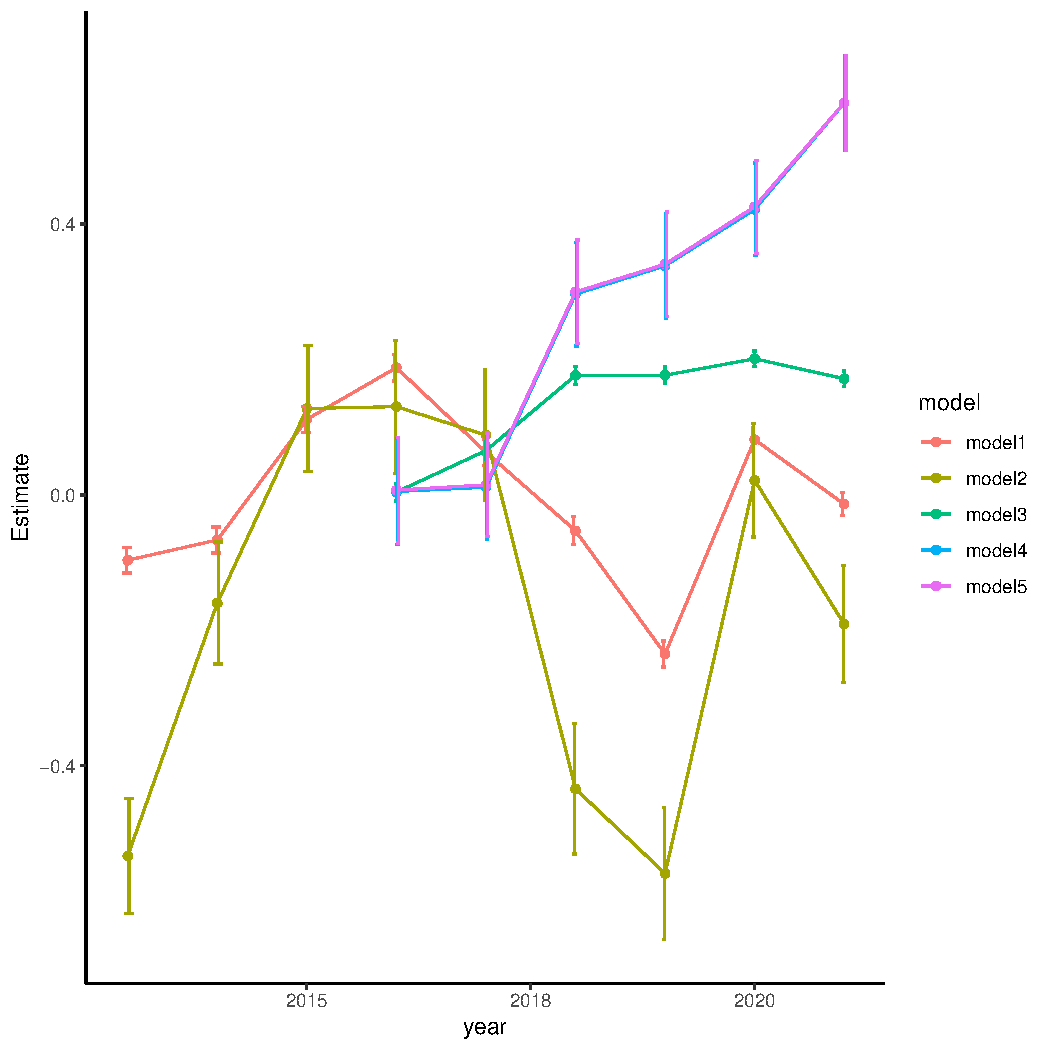
\includegraphics{yearly_plots.pdf}
  \caption{Model Coefficient values for Year, with standard error bars.}\label{fig:yearly}
  \end{figure}

% Search for where you mention quality and where you mention value as this does become misleading!!!
%
% This is partly because of the intercept
%
% It depends what else is in the model.
%
% This direct comparisons are 
%
% The correlated between input vars needs to be discussed earlier.
%
%difference between the continuous variables coefficients is the change from positive to negative values. This change occurs between the Models for Yield (Model 1 and 2) and the Models for value (Models 3 and 4); where all but the coefficient for area harvested had the opposite sign (see Table \ref{tab:contvar}). These models also differ in an order of magnitude when looking at resource use, with the coefficients for yield being smaller than those for value. 
%
% The resource input is different by an order of magnitude between value and yield
%
% Area has the strongest nfluence
%
% The models as a ratio of area show opposite trends - this could be indicative that smaller vineyards tend twoards more valuable crops and larger to crops of greater yield. 
%

Regional differences are summarised in Figure \ref{fig:spider}. The most notable difference is between vineyards within 'Hot' and 'Very Dry' regions (warm inland regions), where high average sale prices are historically low, and yield is high. Water Use changes dramatically between these regions as well, with water being a driving force for yield but not necessarily average sale price. The warmer and drier regions tend to also have larger vineyards.
\par
\begin{figure}
  \resizebox{\textwidth}{!}{
  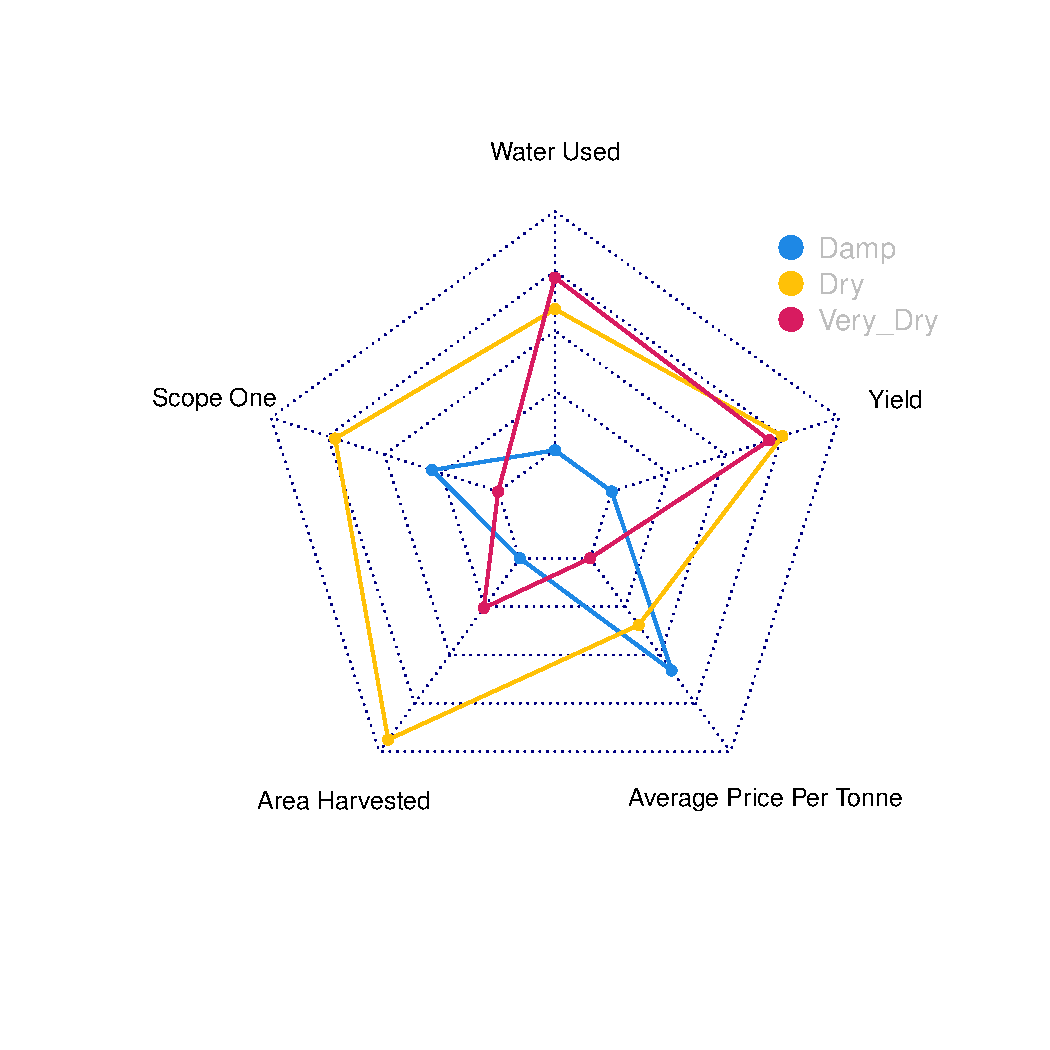
\includegraphics{starplots.png}}
  \caption{Radar plot of climatic profile's resource use, yield and average sale price. The left reflects vineyards in different climatic temperatures. The right reflects vineyards in different rainfall climates.}\label{fig:spider}
\end{figure}

Figure \ref{fig:yield_vs_value_area} further shows the emphasis that 'Hot' areas have on high yields with low average sale price compared with other regions. Scaling average price and yield by area shows a strong negative trend, trading quantity for higher sales prices.
\par
\begin{figure}
  \resizebox{\textwidth}{!}{
  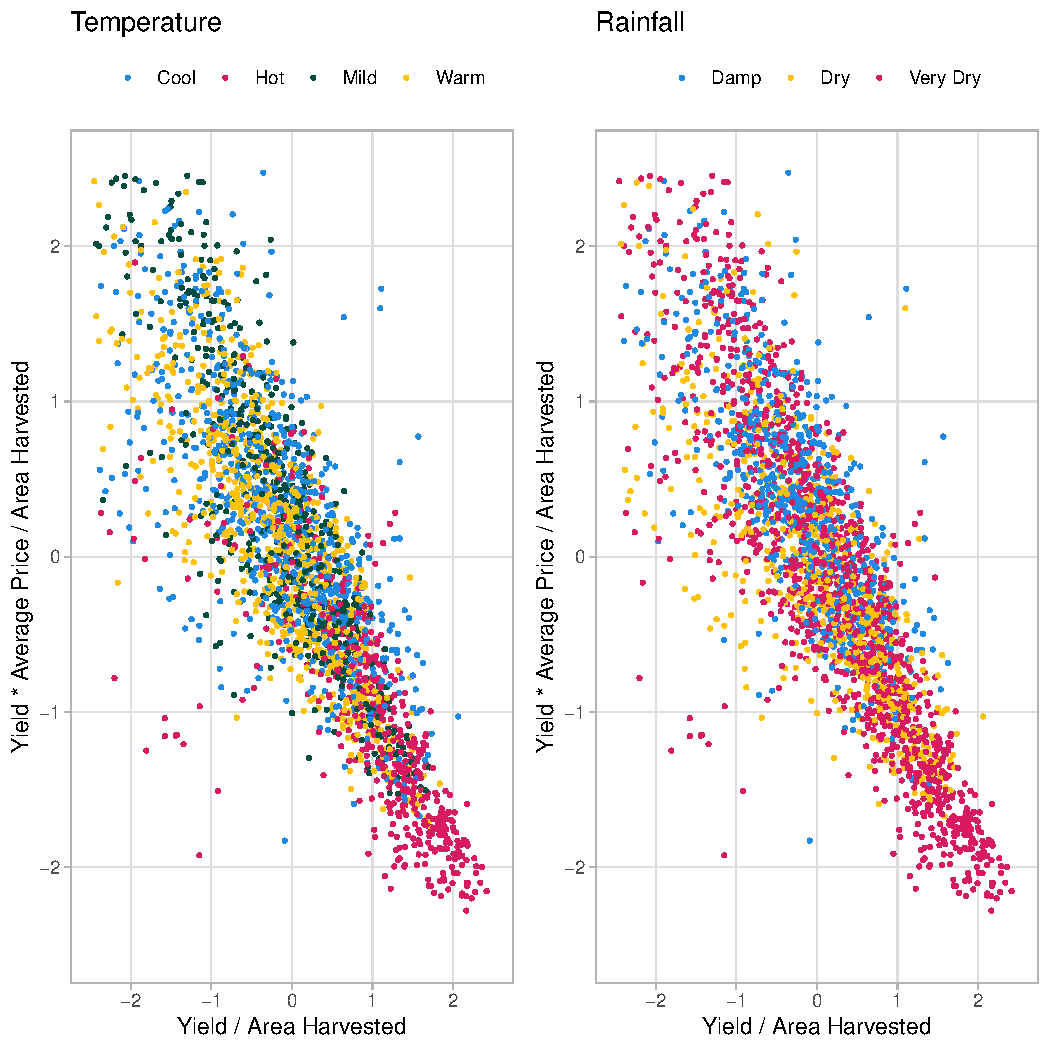
\includegraphics{yield_verse_value_by_area.pdf}}
    \caption{Scatter plot of vineyard yield against the average sale price as ratios to area harvested. The axes are in standard deviations with points coloured by climate.}\label{fig:yield_vs_value_area}
\end{figure}

Table \ref{tab:kfold} shows the validation results of each of the models. The $R^2$ measures of fit show similar results to the initial models, with a slight decrease. Indicating that the models are robust and consistent.
%
%
% At least summary statistics of the baseline model.
%
%
\par
\begin{table}[]
  \label{tab:kfold}
  \caption{Model validation using k-fold cross validation, for 10 folds repeated 100 times.}
  % \resizebox{\textwidth}{!}{
  \begin{tabular}{@{}cccc@{}}
    \toprule
    \textbf{} & \textbf{\begin{tabular}[c]{@{}c@{}}Residual Mean\\ Squared Error\end{tabular}} & \textbf{R2} & \textbf{\begin{tabular}[c]{@{}c@{}}Mean Average \\ Error\end{tabular}} \\ \midrule
    \textbf{Model 1} & .309 & .905 & .2165 \\
    \textbf{Model 2} & .457 & .7921 & .313 \\
    \textbf{Model 3} & .165 & .972 & .101 \\
    \textbf{Model 4} & .348 & .878 & .182 \\ 
    \textbf{Model 5} & .348 & .878 & .183 \\ \bottomrule
    \end{tabular}
  % }
  \end{table}

\section{Discussion}

There was an expected strong relationship between size and resource use, with the overall area of a vineyard and its access to resources greatly determining the upper limit of potential yield. However, size was also inversely related to the potential average sale price, with higher sales prices being related to high resource inputs per area; rather than to the overall expenditure of resources. Vineyard yields and sales price changed greatly by region and year. Even given regional and yearly changes, there was a strong connection between smaller vineyards and higher sales prices. This could have been due to more attention available when managing smaller properties.
\par
The lack of significance of scope one emissions and its contribution to models, given its F-statistics, could be indicative that other vineyard activities requiring fuel are not leading factors for a vineyards avereage sale price. The relationship between yield, value and area was not simply about efficiently producing the most grapes. It is possible that the relationship of scope one emissions between yield and sale price was closely tied to a vineyard's area due to requiring more fuel to address more issues over greater distances. It is difficult to discern the connection of scope one emissions directly, as fuel can be used for a broad category of activities. 
\par
There are important considerations unique to winegrowing compared to other agricultural industries. The vertical integration of winegrowing within the wine industry ties winegrowers to secondary and tertiary industries, such as wine production, packaging, transport and sales. This results in unique issues and considerations for each vineyard, where on-the-ground decisions are influenced by other wine industry's choices, such as the use of sustainable practices in vineyards as a requirement for sale in overseas markets; notably these interactions can be further complicated by some winegrowers being completely integrated into a wine company, while others are not \citep{knightFirmResourcesDevelopment2019}. Incorporating decisions into the model could help describe the contributing factors to regional differences beyond resource consumption, motivating the call for more granular data and more sophisticated modelling.
\par
There are many on-the-ground decisions that influence both sales price and yield. The decision to prioritise average sale price over quantity, is governed by complex physical and social forces, for example international market demands, disease pressures and natural disasters \citep{abadCoverCropsViticulture2021,cortezUsingDataMining2009,hallWithinseasonTemporalVariation2011,i.goodwinManagingSoilWater2009,kasimatiPredictingGrapeSugar2022,oliverReviewSoilPhysical2013,srivastavaNondestructiveSensingMethods2018}, with many of these occurrences being highlighted throughout the reports from Wine Australia \citep{wineaustraliaNationalVintageReport2019,wineaustraliaNationalVintageReport2021,wineaustraliaNationalVintageReport2022,winemakersfederationofaustraliaNationalVintageReport2013,winemakersfederationofaustraliaNationalVintageReport2014,winemakersfederationofaustraliaNationalVintageReport2015,winemakersfederationofaustraliaNationalVintageReport2016,winemakersfederationofaustraliaNationalVintageReport2017,winemakersfederationofaustraliaNationalVintageReport2018} over the past decade. However, the changes in the coefficients (see Figure \ref{fig:yearly}) are not reflective of many known occurrences, such as the 2020 bush fires, which had higher values for coefficients than prior years; During the 2020 bush fires 40,000 tonnes of grapes were lost across 18 different wine regions due to bush fires and smoke taint. In comparison to countrywide pressures such as drought, this damage made up only 3\% of the total amount of grapes for that year; although acknowledged as a considerable loss on an individual basis, it was deemed to be only a minor national concern by Wine Australia when compared to other environmental pressures such as drought \citep{wineaustraliaNationalVintageReport2020}
\par
Climatic pressures are an important consideration for growers, especially those in warmer and drier regions. The Wine Australia reports also show that warm inland regions have seen a decline in profit over the past decade, whereas regions with lower avereage sales prices did not \citep{wineaustraliaNationalVintageReport2019,wineaustraliaNationalVintageReport2020,wineaustraliaNationalVintageReport2021,winemakersfederationofaustraliaNationalVintageReport2013,winemakersfederationofaustraliaNationalVintageReport2014,winemakersfederationofaustraliaNationalVintageReport2015,winemakersfederationofaustraliaNationalVintageReport2016,winemakersfederationofaustraliaNationalVintageReport2017,winemakersfederationofaustraliaNationalVintageReport2018}. Vineyards in warm inland regions also tend to contain larger vineyards, making up for lower sale prices with larger yields. Considering the negative correlation of average price to area, for this strategy to work, economies of scale become and important factor. Given the large quantities of grapes that can be produced by some vineyards, even at low margins there is the potential to be profitable. However, the increasing climatic pressures mixed with the requirement for larger volumes of water, make the sustainability of some vineyards come into question. Furthermore, intensive farming in general is known to jeopardise the sustainability of an operation through the degradation of soil and waterways \citep{capelloEffectsTractorPasses2019,linHydropedologySynergisticIntegration2012,pisciottaGroundwaterNitrateRisk2015}. There are established methods that can help to mitigate these effect, such as the use of cover crops and midrow crop rotation. However, it has become more apparent that the active reduction of grape yield, through methods such as thinning, can help improve soil health \citep{condursoEffectsClusterThinning2016,wangChangesGlobalAroma2019}.
\par
Some regions appeared to produce grapes of lower average sale price at scale whilst others focussed on producing higher priced grapes in lower volumes. This empirical finding is consistent with Wine Australia's annual reports, which shows that some GI regions, such as the Riverland, are known for producing large amounts of lower grade (low value per tonne) grapes \citep{wineaustraliaNationalVintageReport2022,winemakersfederationofaustraliaNationalVintageReport2017}. Comparatively, other regions, such as Tasmania, only produce grapes of higher sales price but in smaller quantities. The difference in pricing per tonne between the lowest and highest graded grapes can be greater than a hundred times the difference in value per tonne. Not all regions target only one grade of grape, with some producing a variety of differently graded grapes; such as the Yarra Valley, which produces grades from C to A. This effect could stifle the potential for market opportunities within lesser known regions. A further possibility is the existence of regional upper limits on potential sales price, or that there are diminishing returns in some regions when pursuing higher sales prices or quantity; however these types of relationships may be obfuscated by knowledgeable winegrowers who avoid this pitfall.
\par
Due to regional differences, different strategies are also  employed across different regions, such as some regions targeting mass production over higher sales price. This is most notable when grouping regions by climate, especially when considering GI Regions in the 'Hot Very Dry' climate (see Figure \ref{fig:yield_vs_value_area}). 
%In the preliminary analyses alternative models found that without the direct incorporation of GI Region or year, predictions greatly under performed. The effect of climate in the models was never as significant as the more granular GI regions, and always led to less accurate models. 
Although not chosen over GI region, climate was considered to be a large determinant of the ability to produce larger quantities of grapes, as well as a determinant in grape sale price \citep{agostaRegionalClimateVariability2012}. The more granular GI Region likely explained a broader mix of geographical phenomenon, such as soil, geology and access to water resources \citep{abbalDecisionSupportSystem2016,carmonaUseParticipatoryObjectOriented2011}. The interaction between year and GI Region likely accounted for events such as bushfires, which would be impactful, but only at a local level, both in time and space.
\par
We identified two main limiations to our linear modeling. First model 1 and 2 over-predicting yield may have been due to preventative measures brought on by regional pressures such as fire, frost and disease. More fuel and water was likely used to prevent these issues from spreading within a region, thus disproportionately affecting some vineyards compared to others locally. This type of maintenance is not well captured in the models, especially when considering that some regions, especially those in warmer areas, are not as prone to disease as cooler climates and could potentially have lower fuel and water use per hectare. This could create a discrepancy in vineyards that utilised preventative measures in wetter regions, as opposed to those that did not, thus expending less fuel and energy but risking disease. When reviewing the differences between regions, it is important to consider that vineyards in 'Hot Very Dry' areas can be hundreds of times the size of those in other regions. This limitation could be overcome by incorporating the profitability of vineyards, comparing the financial success of working at different operational scales.
\par
The second limitations was the lack of further explanatory variables to help link models to causal affects. Variables such as the utilisation of renewable energy, contractors, and the occurrence of disease, fire and frost were originally explored to capture the discrepancies between similar vineyards that produced different yields and crop values. However, none of these variables was significantly correlated with the response variables, and did not add to model accuracy, even when considered as interactions. Allowance for nonlinear relationships, specifically through splines, resulted in more normally distributed residuals but at a drastically reduced overall accuracy when comparing $R^2$ and Residual Square Error. Attempts to fully explain small variations was always overshadowed by the dramatic differences in regional trends. Having more data for each region would also be beneficial, allowing greater comparison between regions. More variables, such as soil quality and health, may also help to discern vineyards that can produce larger volumes of grapes at higher prices.
\par
The use of other models such as random forests and decision trees alongside more variables and data may help to uncover the reasons for under or overestimation. These differences could be caused by the use of alternative sustainable practices in the field. Moreover, while there is evidence to suggest that environmentally sustainable practices can reduce costs, and increase efficiency whilst improving the quality of grapes; more research is needed to link these benefits across different regions and climates \citep{baianoOverviewSustainabilityWine2021,marianiSustainableWinegrowingCurrent2015,montalvo-falconSustainabilityResearchWine2023}.
\section{Conclusion}

This study delved into the relationships between resource use, grape sales price and yield. The findings underscore the multifaceted nature of vineyard management, where the interplay of size, resource allocation, climate, and regional influences collectively shape both the expected sale price and the quantity of grape yields. Average sales price of grapes was not solely tied to the overall expenditure of resources, but rather to the efficient allocation of resources per unit area. This emphasises that factors beyond sheer scale contribute significantly to the final sale price of grapes produced. Moreover, regional and yearly variations exhibited substantial effects on vineyard outputs, impacting both sales price and quantity. The connection observed between smaller vineyards and higher grape sale price suggests that the management of smaller properties might be more streamlined and effective.


\bibliography{references}
\bibliographystyle{elsarticle-harv}

%% The Appendices part is started with the command \appendix;
%% appendix sections are then done as normal sections
 \appendix

\section{Appendix}
\par

\begin{table}[]
      \caption{P-values for the non-transformed water used variable's Pearson correlation coefficients.}
      \begin{tabular}{cl}
      Variable                                           & Water Used \\
      Yield                                              & 7.538E-01  \\
      Area                                               & 6.981E-01  \\
      Scope One Emissions                                & 8.883E-01  \\
      $\textrm{Yield}\over\textrm{Area}$                     & 6.836E-01  \\
      Average Price Per Tonne                            & 5.600E-02  \\
      ${\textrm{Average Price per tonne}\over\textrm{Area}}$ & 1.522E-01 
      \end{tabular}
\end{table}


\begin{figure}
  \resizebox{\textwidth}{!}{
  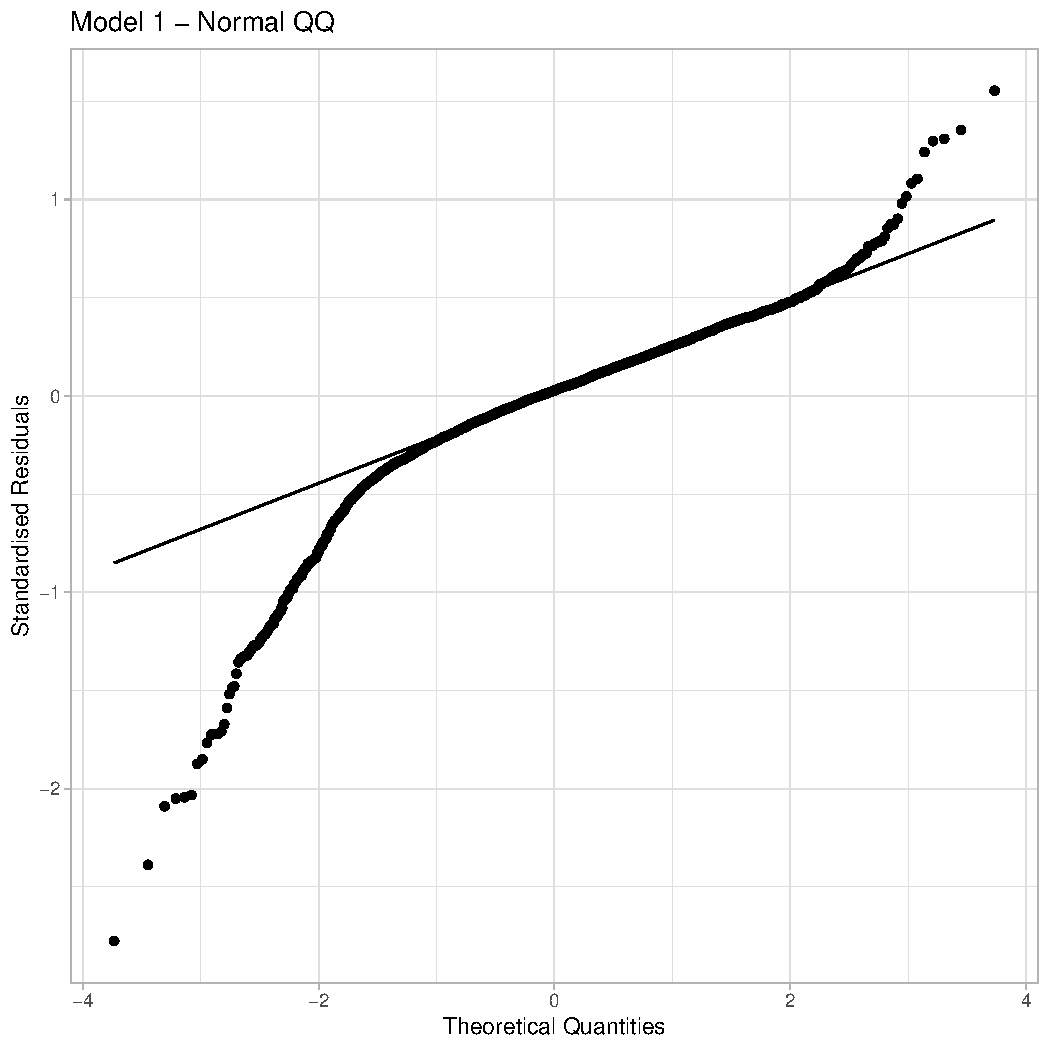
\includegraphics{model1_qq.pdf}}
  \caption{QQ-plot of Model 1.}
\end{figure}

\begin{figure}
  \resizebox{\textwidth}{!}{
  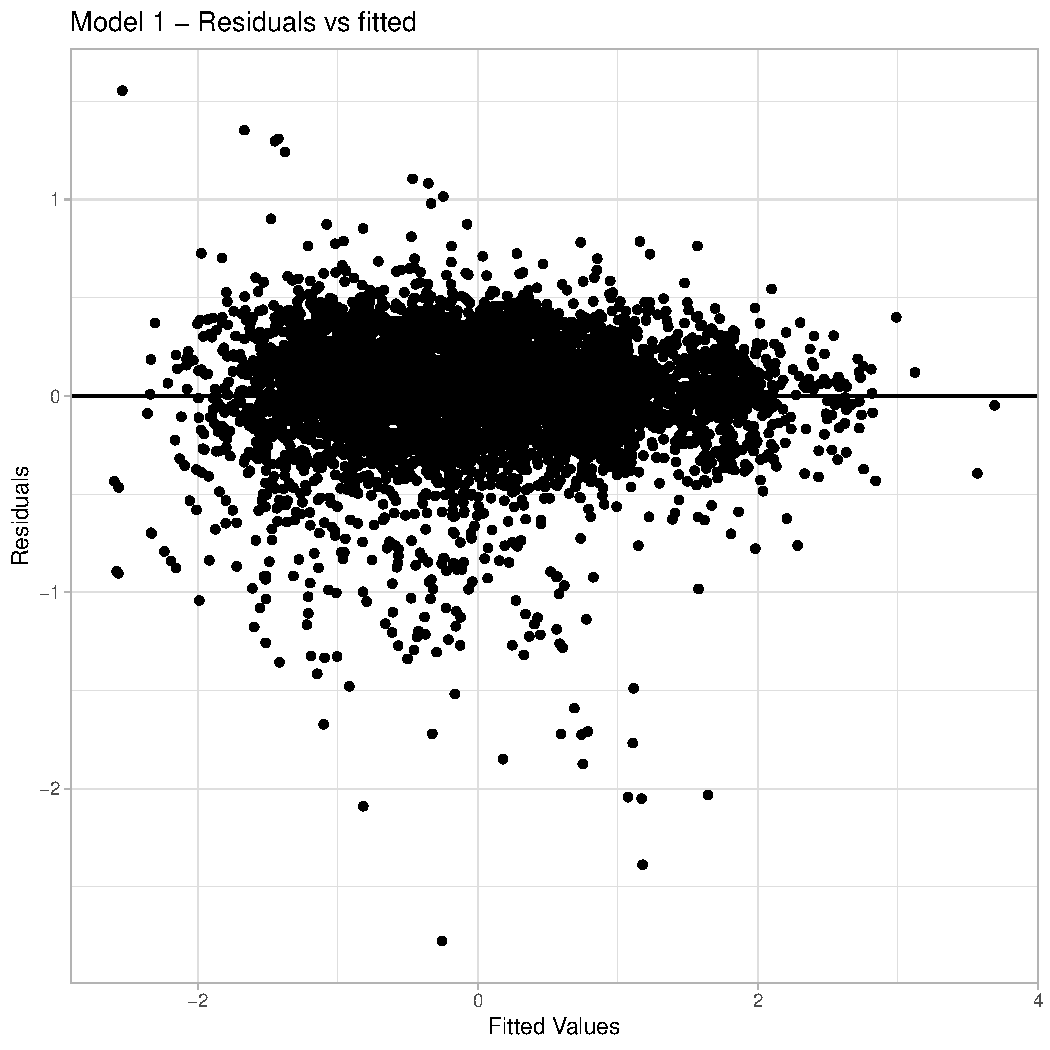
\includegraphics{model1_rvf.pdf}}
  \caption{Residuals vs fitted values for Model 1.}
\end{figure}

\begin{figure}
  \resizebox{\textwidth}{!}{
  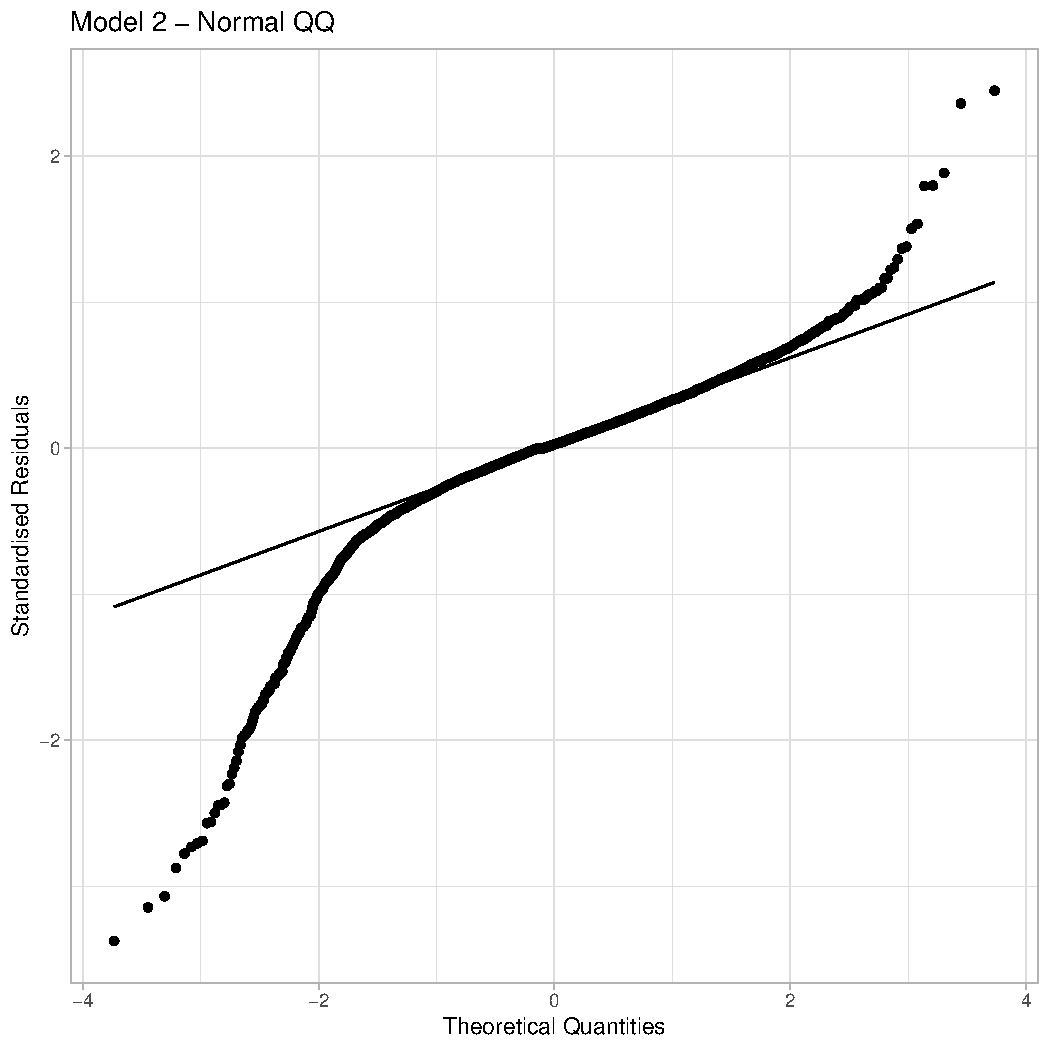
\includegraphics{model2_qq.pdf}}
  \caption{QQ-plot of Model 2.}
\end{figure}

\begin{figure}
  \resizebox{\textwidth}{!}{
  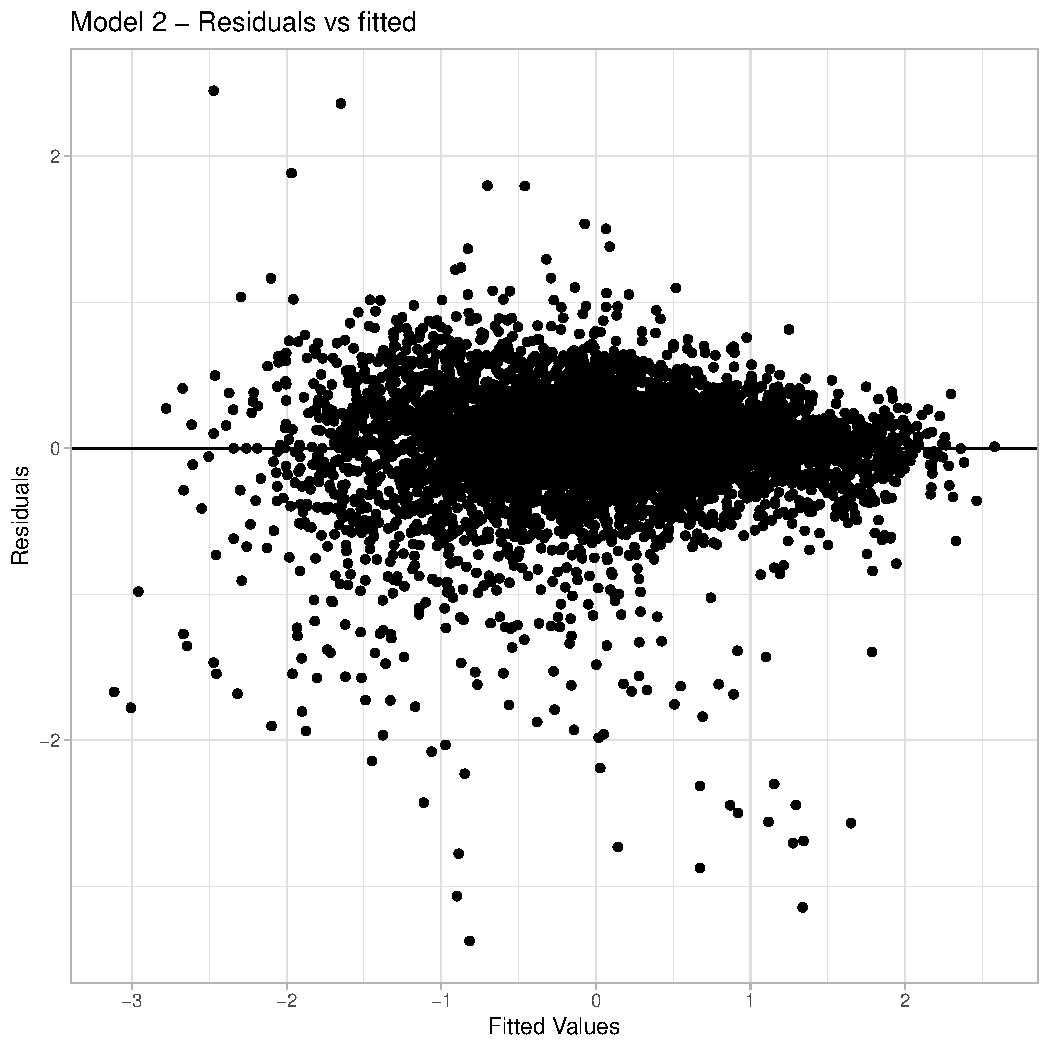
\includegraphics{model2_rvf.pdf}}
  \caption{Residuals vs fitted values for Model 2.}
\end{figure}

\begin{figure}
  \resizebox{\textwidth}{!}{
  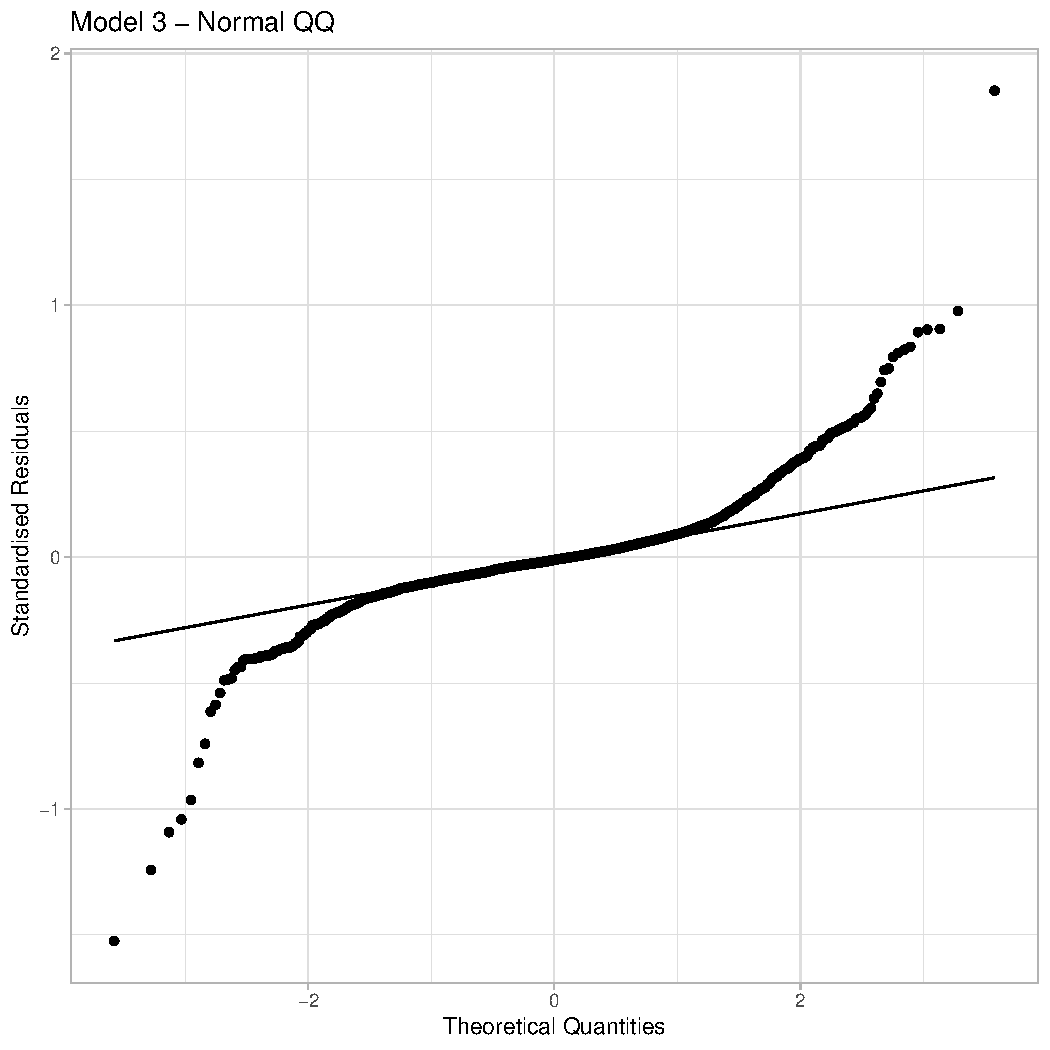
\includegraphics{model3_qq.pdf}}
  \caption{QQ-plot of Model 3.}
\end{figure}

\begin{figure}
  \resizebox{\textwidth}{!}{
  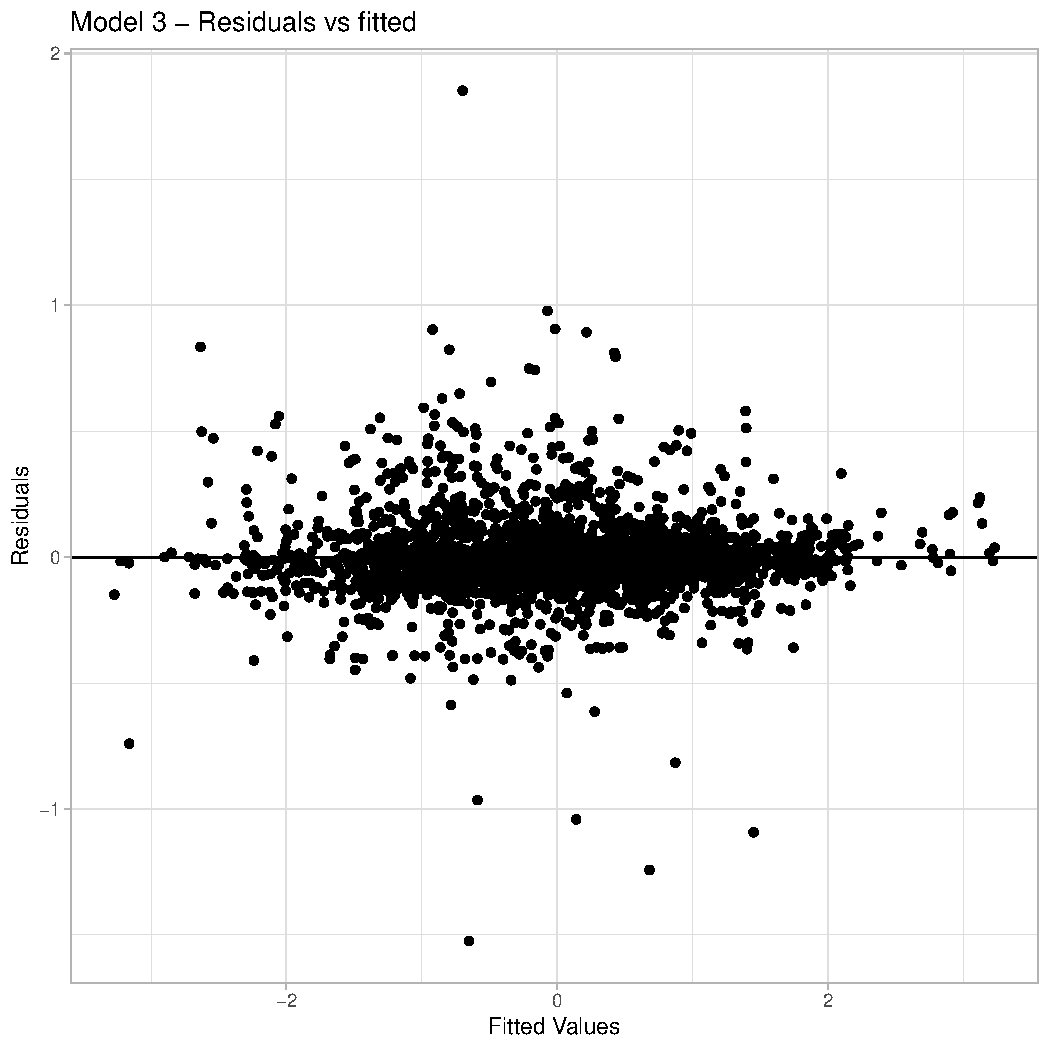
\includegraphics{model3_rvf.pdf}}
  \caption{Residuals vs fitted values for Model 3.}
\end{figure}

\begin{figure}
  \resizebox{\textwidth}{!}{
  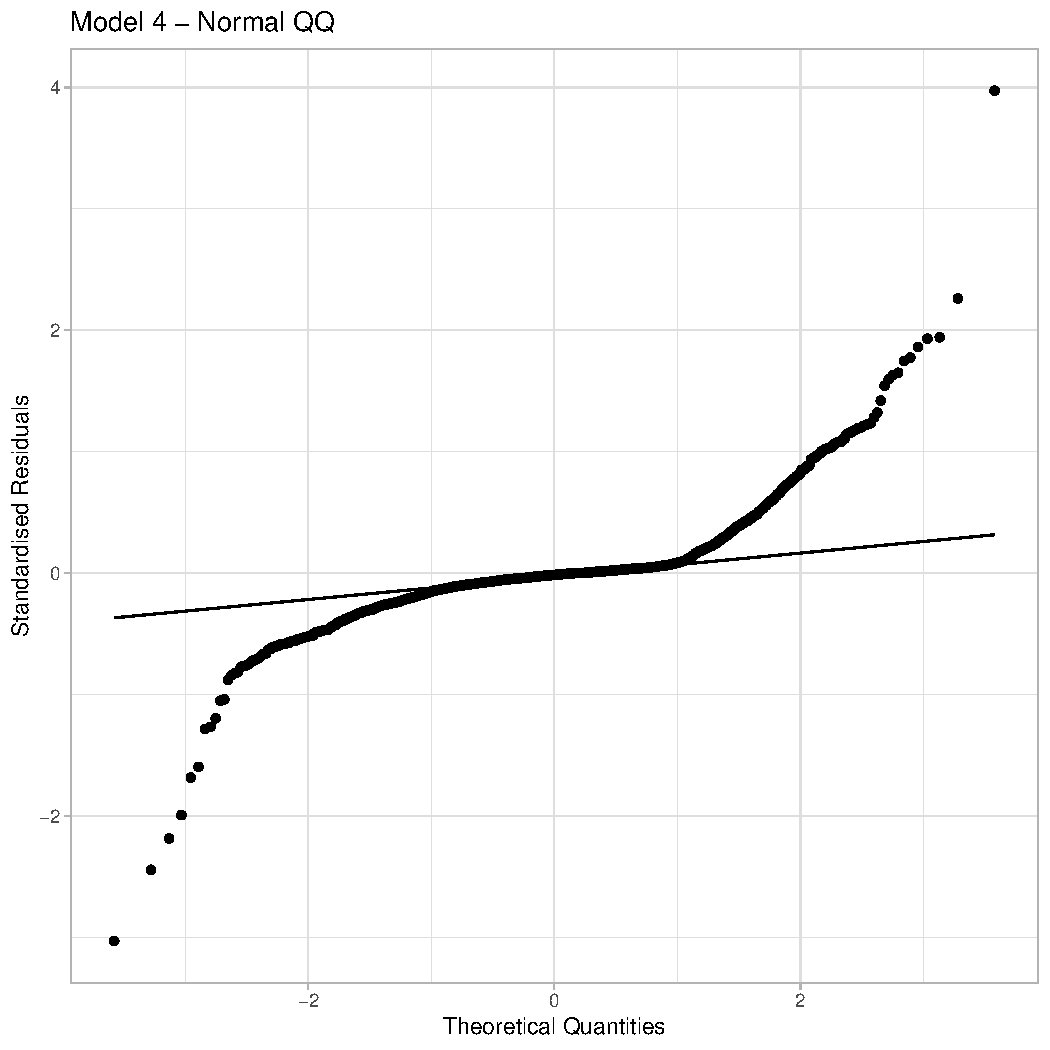
\includegraphics{model4_qq.pdf}}
  \caption{QQ-plot of Model 4.}
\end{figure}

\begin{figure}
  \resizebox{\textwidth}{!}{
  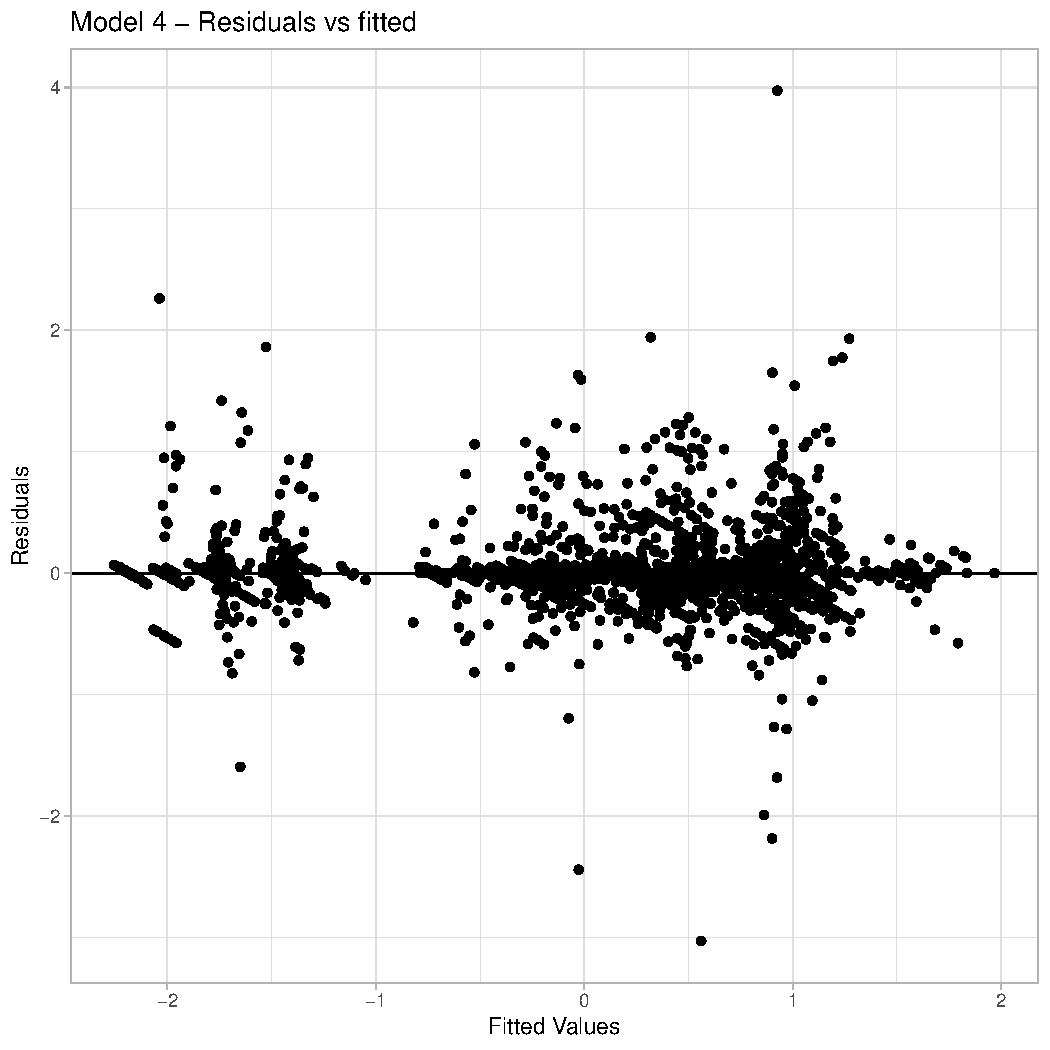
\includegraphics{model4_rvf.pdf}}
  \caption{Residuals vs fitted values for Model 4.}
\end{figure}
\begin{figure}
  \resizebox{\textwidth}{!}{
  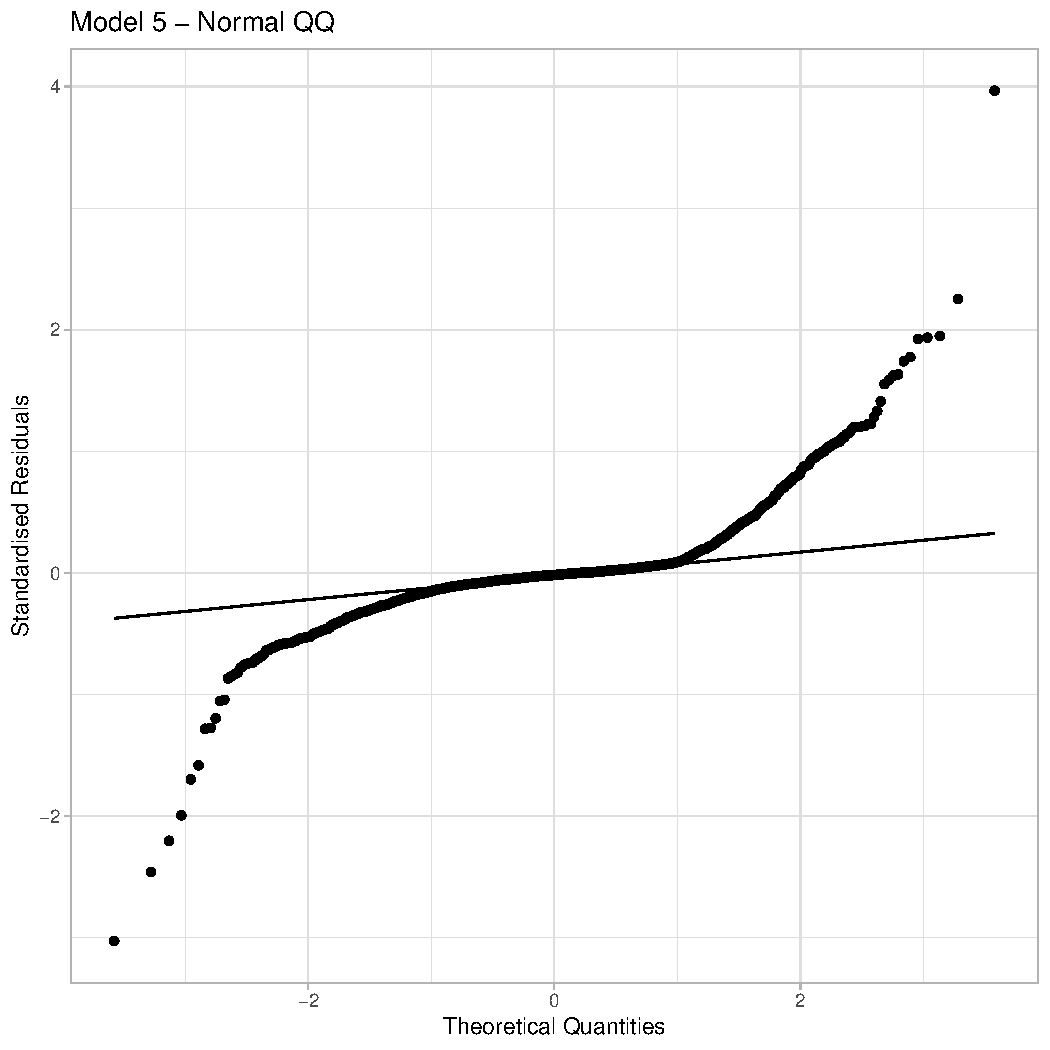
\includegraphics{model5_qq.pdf}}
  \caption{QQ-plot of Model 5.}
\end{figure}

\begin{figure}
  \resizebox{\textwidth}{!}{
  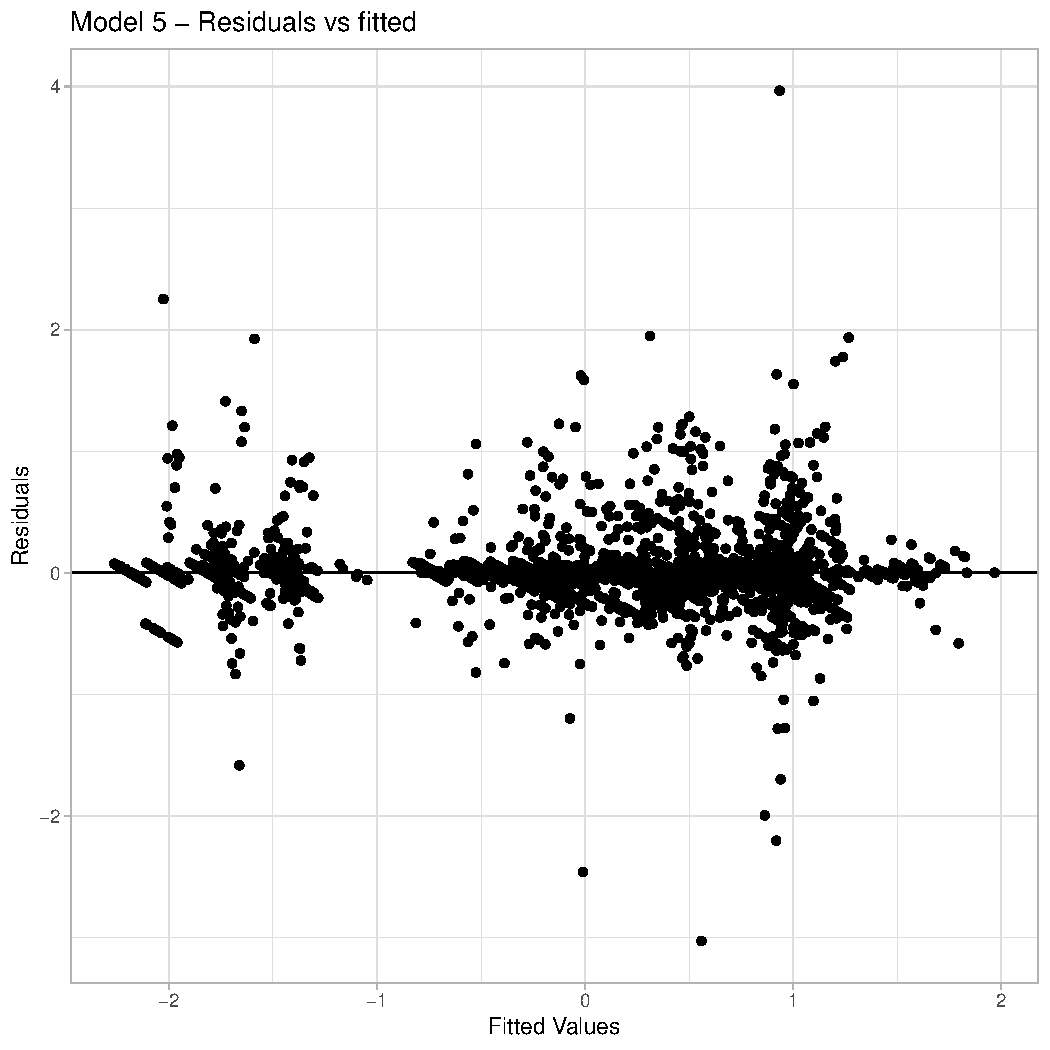
\includegraphics{model5_rvf.pdf}}
  \caption{Residuals vs fitted values for Model 5.}
\end{figure}

% \subsection{Complete list of coefficients for Model 1.}
% \csvautolongtable[]{model1_coef.csv}

%   \subsection{Complete list of coefficients for Model 2.}
% \csvautolongtable[]{model2_coef.csv}


%   \subsection{Complete list of coefficients for Model 3.}
% \csvautolongtable[]{model3_coef.csv}


%   \subsection{Complete list of coefficients for Model 4.}
% \csvautolongtable[]{model4_coef.csv}


%   \subsection{Complete list of coefficients for Model 5.}
% \csvautolongtable[]{model5_coefs.csv}

%
%% \section{}
%% \label{}

%% If you have bibdatabase file and want bibtex to generate the
%% bibitems, please use
%%

%% else use the following coding to input the bibitems directly in the
%% TeX file.

\end{linenumbers}
  \end{document}
  
  \endinput
